\section{Recovery}
\label{sec:recovery}

\subsection{Deployment System}

Recovery is accomplished by a two stage parachute system. At apogee, the nose cone is separated from the body tube via our custom designed clamp band mechanism. It consists of two coupler rings (one mounted to the body tube and the other one to the nose cone) tightly clamped together via a spring steel band.

\begin{figure}[h]
\centering
\subfloat[Clamp band Connection]{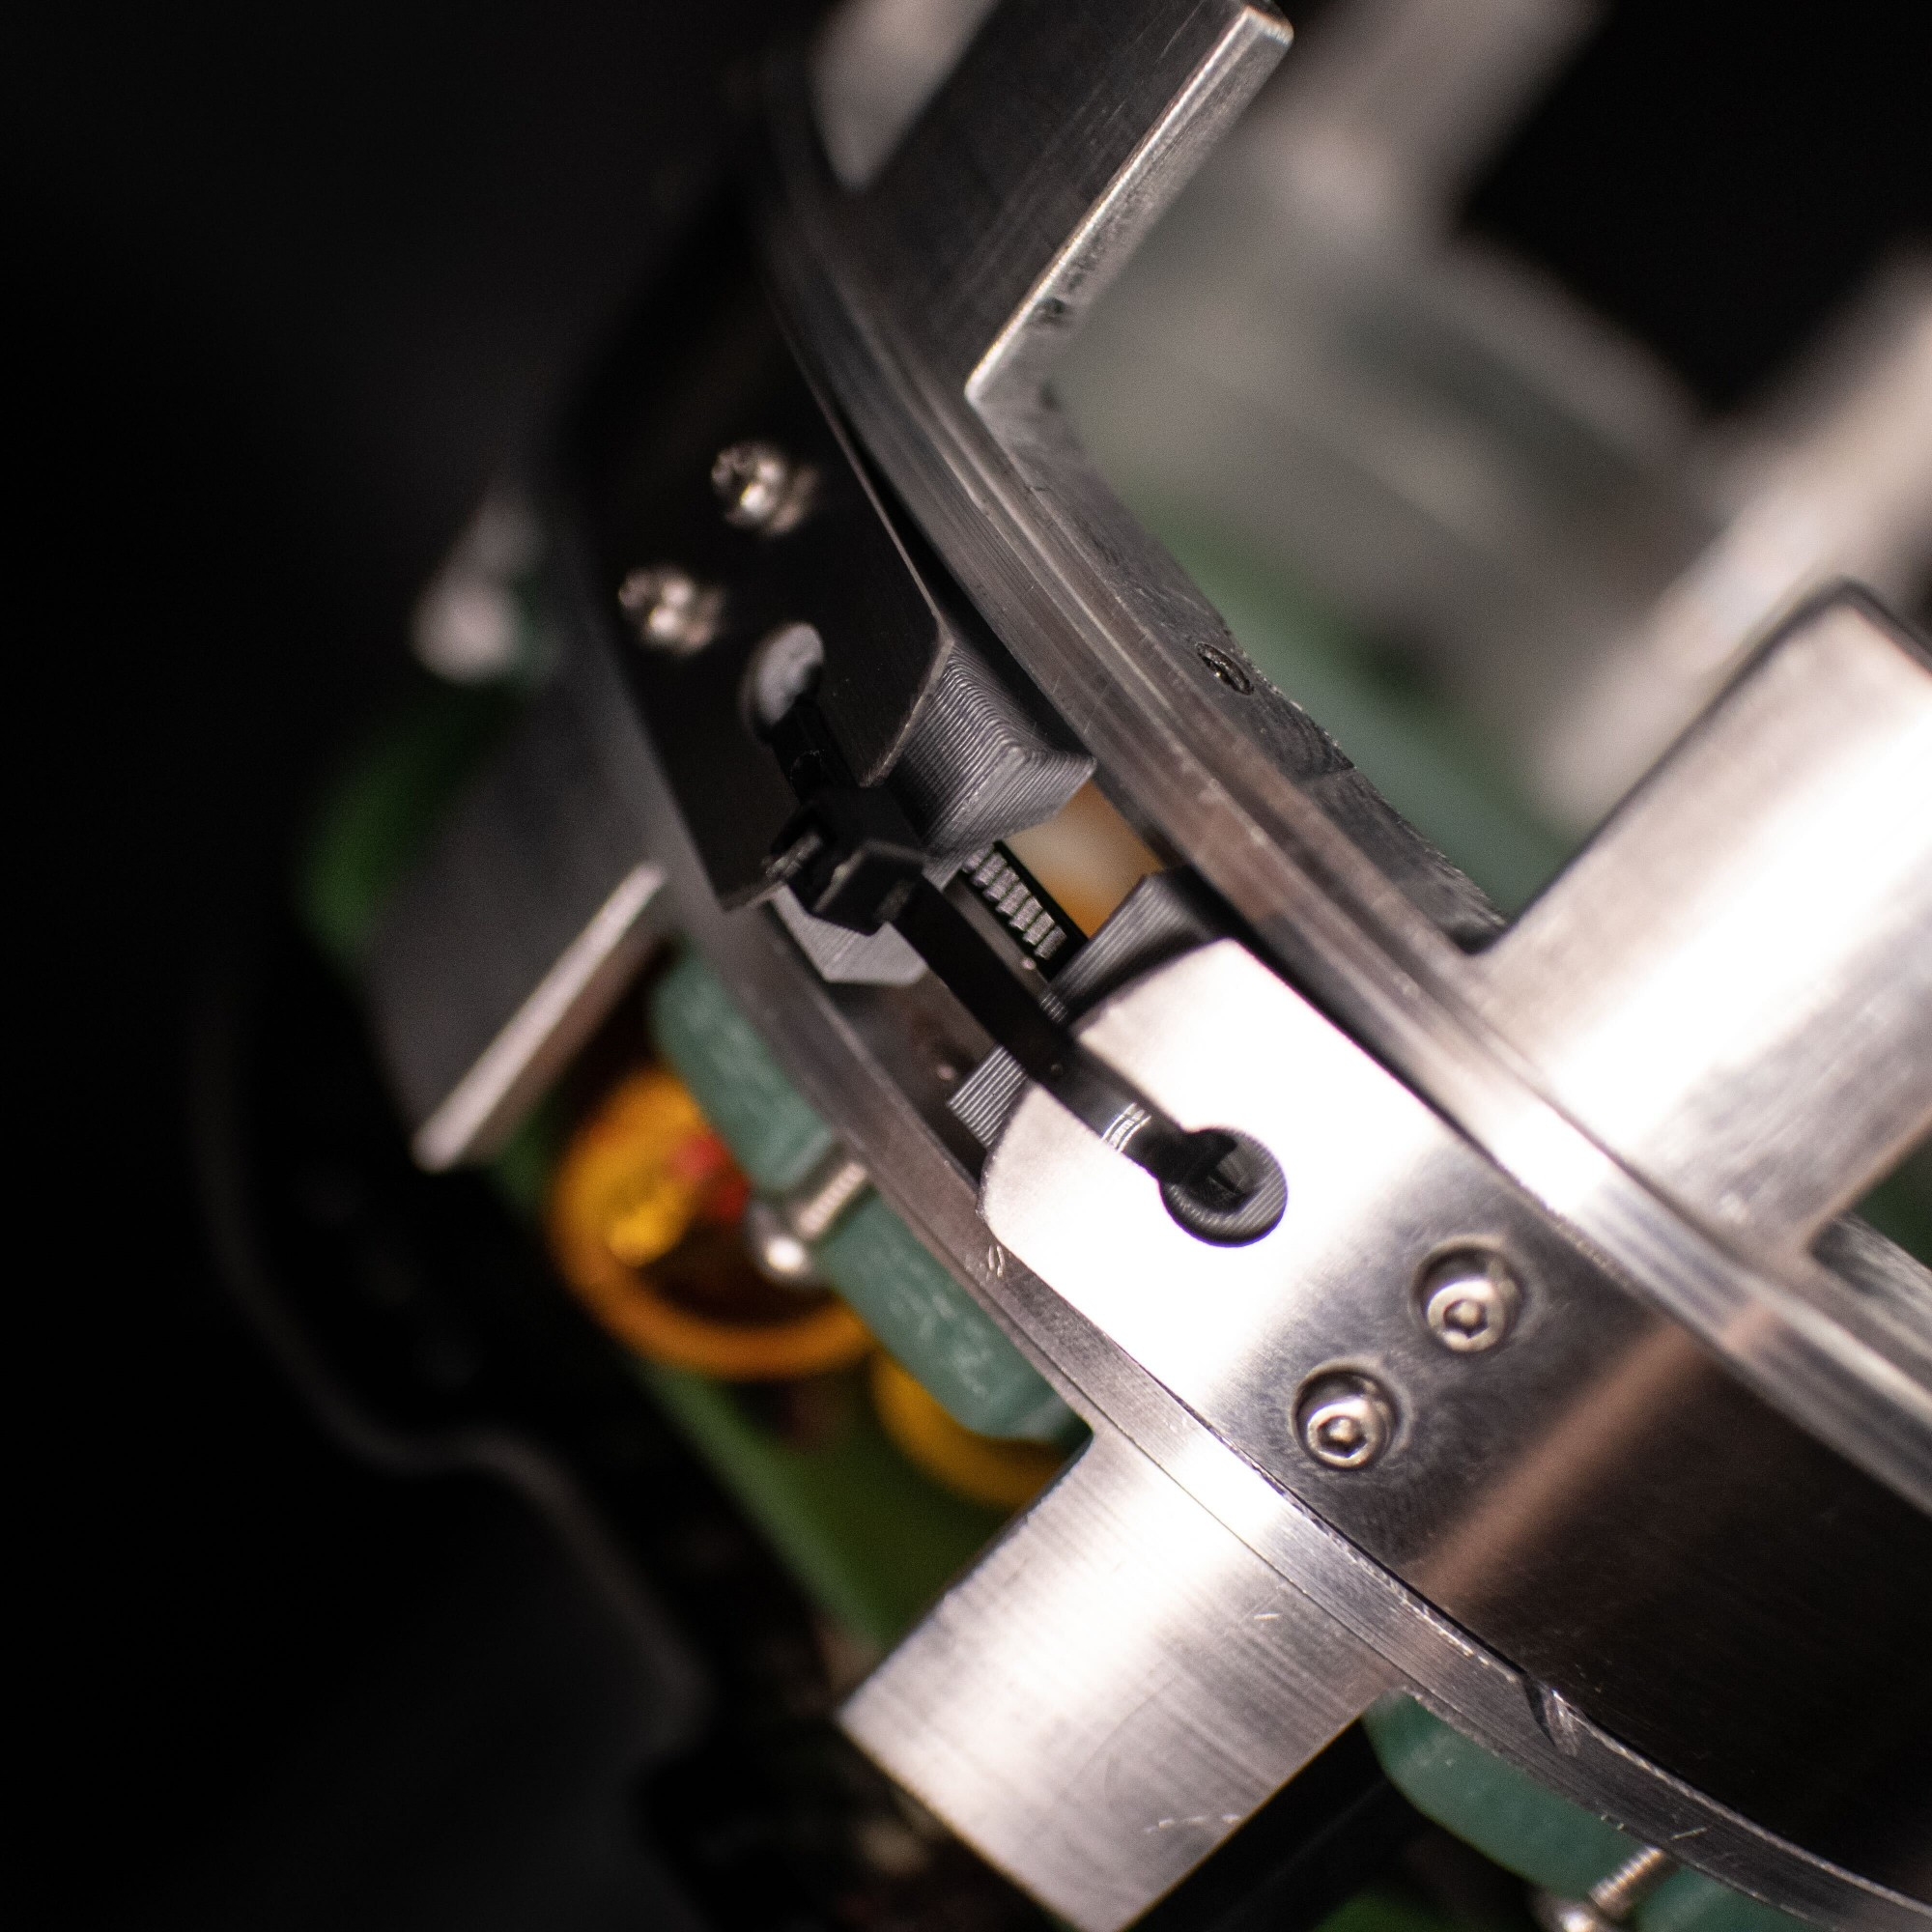
\includegraphics[width=0.4\textwidth]{Recovery/clampband_1.jpg}}
\subfloat[Clamp band coupled to body tube]{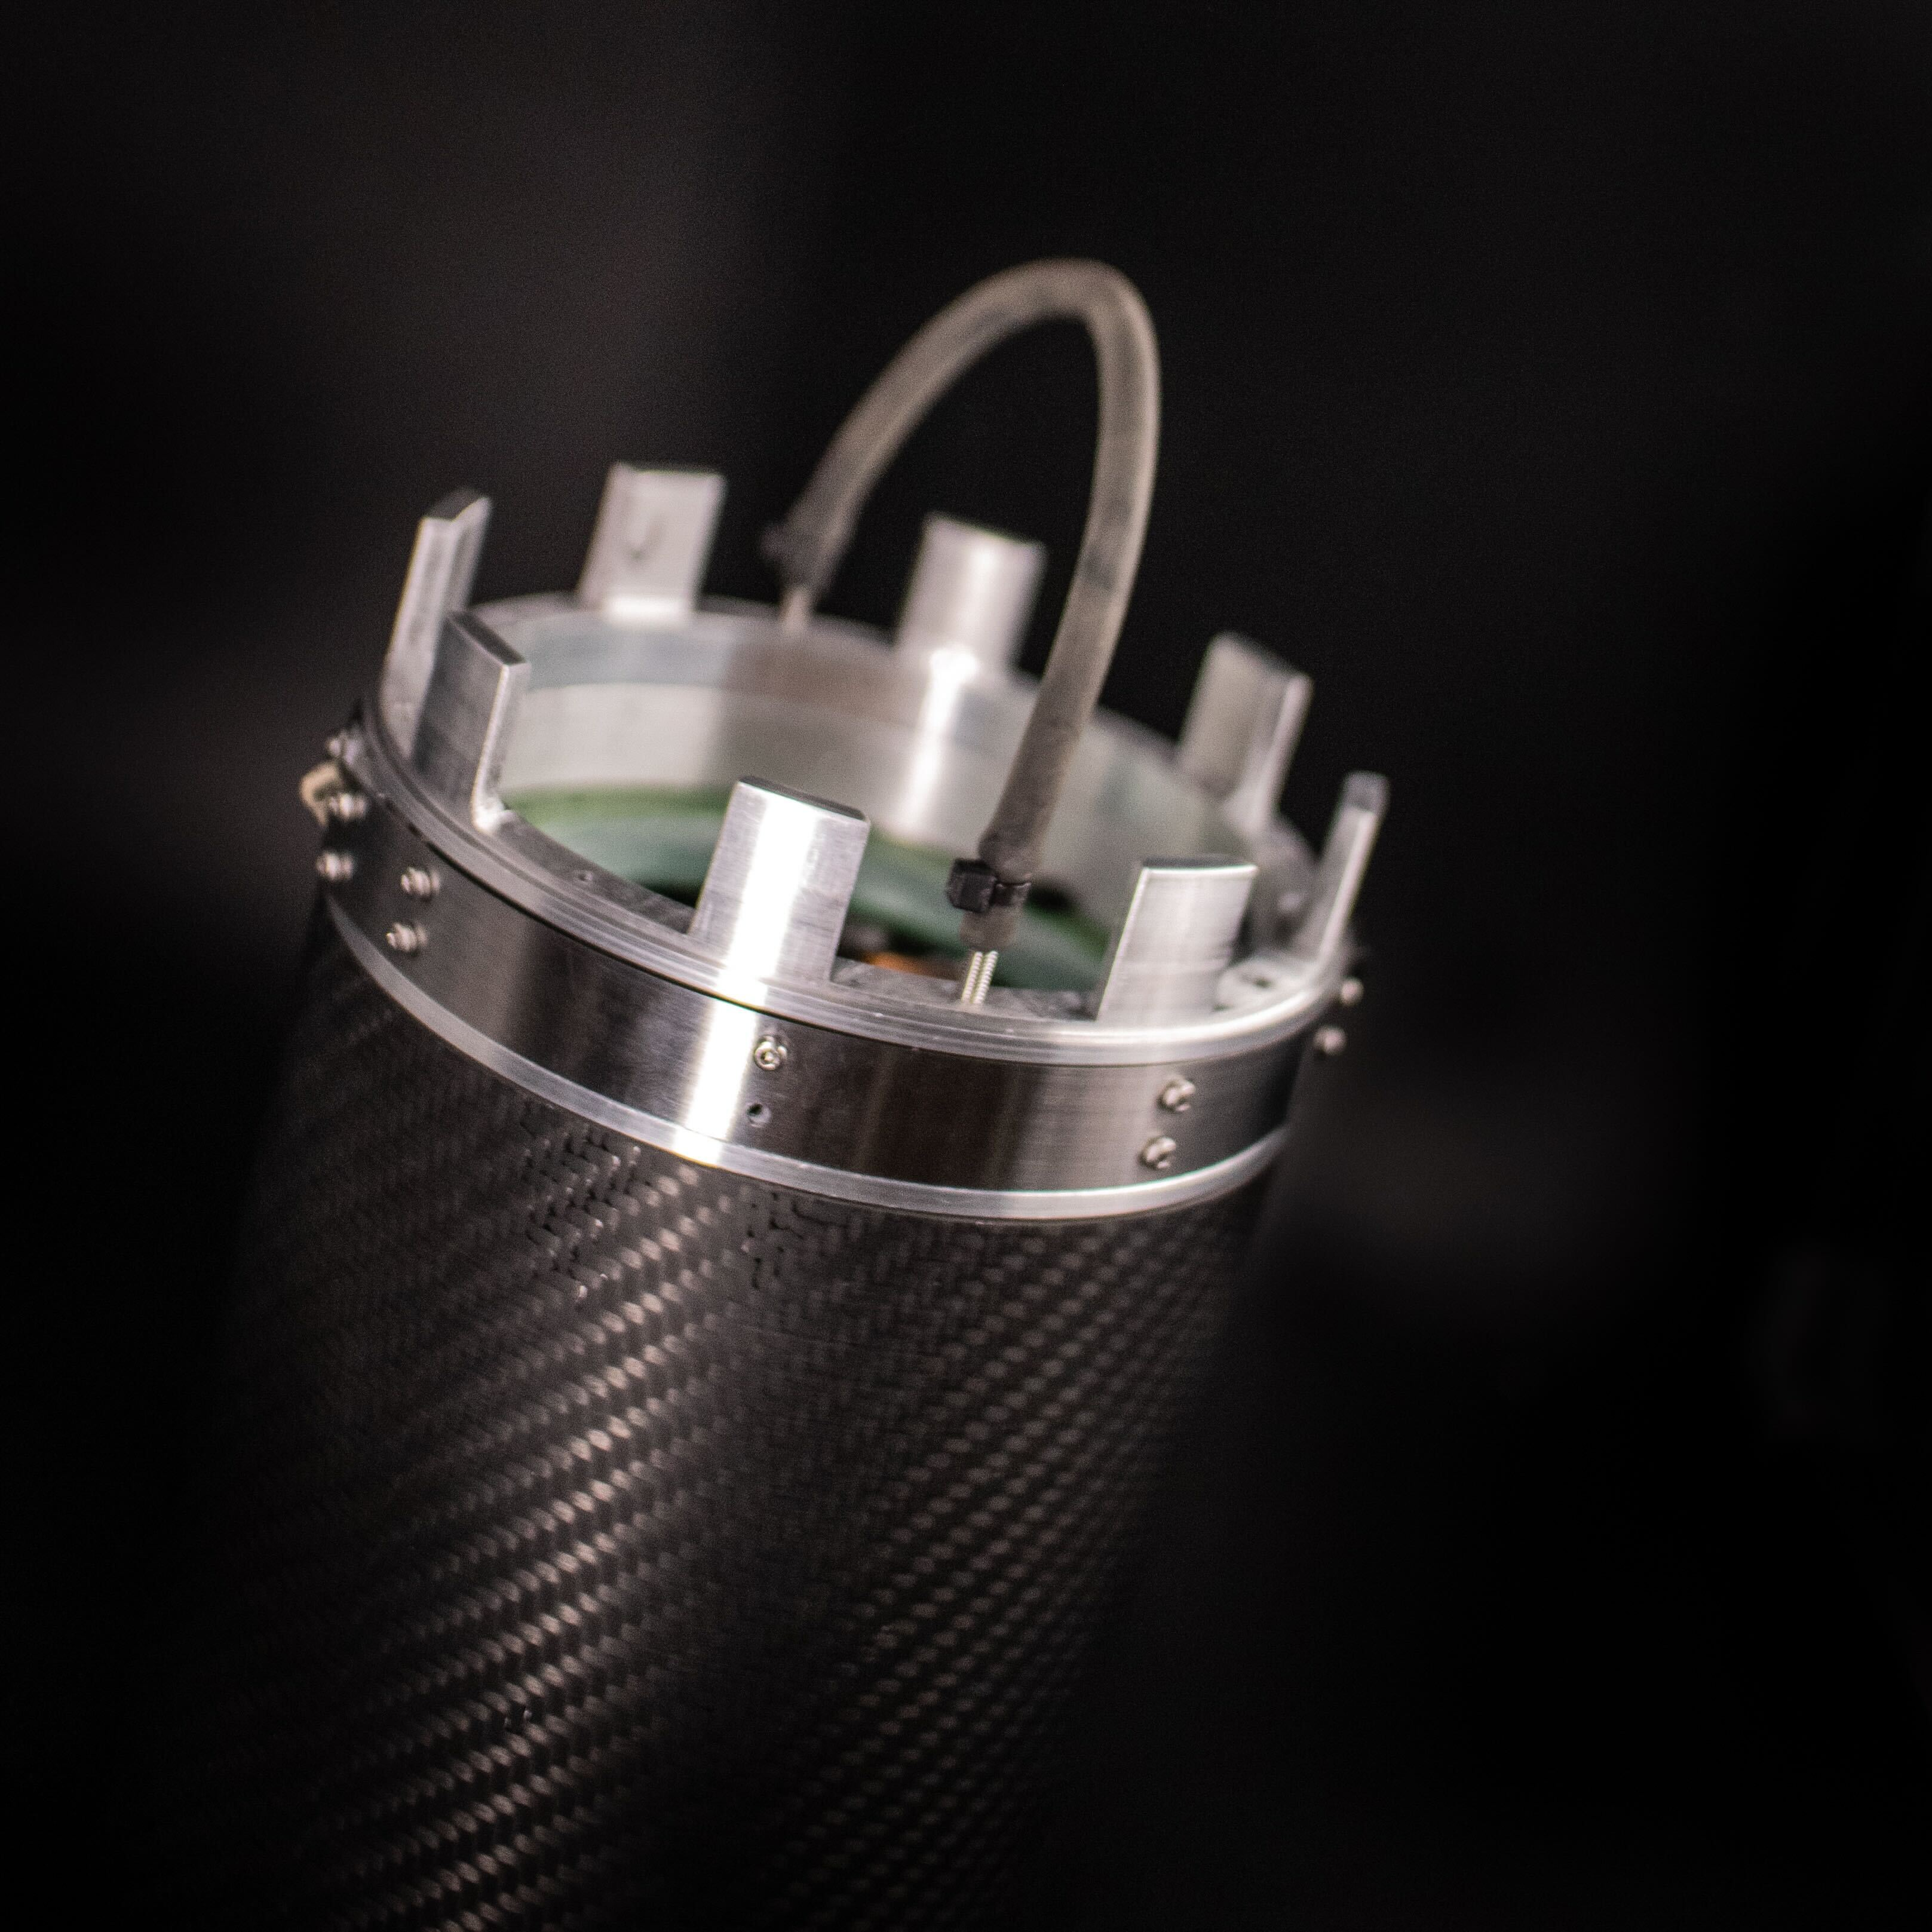
\includegraphics[width=0.4\textwidth]{Recovery/clampband_2.jpg}}
\caption{Clamp band Assembly}
\label{fig:clampband}
\end{figure}

 The clamp band is released by one of two redundant pyrotechnic line cutters severing a line that connects the two ends of the clamp band. The spring steel band separates from the coupler rings (still connected to the main tube by a short line) and releases the connection between them. The coupler on the nose cone is then catapulted away from the bottom coupler ring. This is accomplished by four strong slingshot rubber tubes, ensuring a clean and reliable separation even at high airspeeds (and thus high drag force on the nose cone). Along with the nose cone, a small cup, housing a drogue parachute, is pulled away, releasing the drogue chute.

\subsection{Parachute}

\begin{table}[h]
\centering
\begin{tabular}{ll}
Drogue Chute Diameter & \SI{340}{\milli\meter} \\
Drogue Chute Type & Round \\
Main Chute Diameter & \SI{1400}{\milli\meter} \\
Main Chute Type & Pull-down Apex
\end{tabular}
\caption{Chute Specs}
\label{tab:chute_specs}
\end{table}

During the drogue phase, the vehicle descends quickly (about \SI{35}{\meter\per\second}) and in a controlled manner. The nose cone with the rubber band mechanism and the drogue cup is suspended directly from the drogue with a line shorter than the drogue line to avoid collisions between the nose cone and the body tube. The main parachute and its lines are packed into a deployment bag, which is housed in a cup mounted to the lower section. A few hundred meters above ground, a second set of line cutters severs the connection between the drogue line and the vehicle and another line that keeps the main deployment bag from sliding out of its cup. This puts tension on the line connecting the drogue line and the main deployment bag, allowing the drogue to pull out the main deployment bag. Tension on the main line opens the deployment bag, allowing first the lines and then the parachute to be pulled out of it in a controlled manner. The rocket now descends at about \SI{7.6}{\meter\per\second}.
In this final landing configuration, the drogue and nose cone assembly stay connected to the deployment bag and main parachute. The system has been successfully validated in multiple ground tests, and in a test launch to \SI{700}{\meter} using a mockup airframe propelled by a solid motor. Small modifications are planned to increase reliability and to allow for easier assembly/preparation. Additionally, the parachute sizes will be adapted to the increased vehicle mass.

\subsection{Failure during Test Flight}
On our most recent test flight of the rocket, the recovery has failed by the drogue chute line ripping during the initial drogue deployment. With the rocket then being in free fall the main chute line never had a chance of holding. After carefully studying the received data and video footage of the test flight, the failure has been identified to most likely be caused by the following: The wind speeds encountered at launch day were higher than expected, leading to a higher horizontal velocity at apogee. This of course means that the airspeed, when deploying the drogue, was higher, increasing the load on the lines. Additionally, quite thin drogue lines were chosen based on pre-existing knowledge and experience within the team, which in conjunction with a drogue that was too large and a non-functional shock absorber lead to the lines snapping.
These issues will be rectified in the new recovery system for EuRoC. Since all of the identified causes of the recovery failing have been eliminated and a successful recovery test flight (not using our liquid propulsion, instead having a dummy solid booster) was conducted, we are confident that the recovery system will perform nominally for our flight at EuRoC.